\subsection{Unterkapitel 1}

%Beispiele
Wie \cite{nachname_2005} berichtet, siehe auch Abbildung \ref{fig:Beispiel.png}, Lorem ipsum dolor sit amet, consetetur sadipscing elitr, sed diam nonumy eirmod tempor invidunt ut labore et dolore magna aliquyam erat, sed diam voluptua. At vero eos et accusam et justo duo dolores et ea rebum. Stet clita kasd gubergren, no sea takimata sanctus est Lorem ipsum dolor sit amet. Lorem ipsum dolor sit amet, consetetur sadipscing elitr, sed diam nonumy eirmod tempor invidunt ut labore et dolore magna aliquyam erat, sed diam voluptua. At vero eos et accusam et justo duo dolores et ea rebum. Stet clita kasd gubergren, no sea takimata sanctus est Lorem ipsum dolor sit amet. Lorem ipsum dolor sit amet, consetetur sadipscing elitr, sed diam nonumy eirmod tempor invidunt ut labore et dolore magna aliquyam erat, sed diam voluptua. At vero eos et accusam et justo duo dolores et ea rebum. Stet clita kasd gubergren, no sea takimata sanctus est Lorem ipsum dolor sit amet \citep[vgl.][gemäß freundlicher persönlicher Mitteilung]{nachname_2005}.

\begin{figure}[htb] % Wo das Bild gesetzt wird, entscheidet LaTeX nach Typographischen Aspekten. Wenn ein Bild gesetzt werden soll, bevor ein neues Kapitel anfängt, muss nach dem alten Kapitel der Befehl \clearpage eingesetzt werden. Dann werden alle Float-Umgebungen, die noch "in der Luft hängen", gesetzt.
\centering
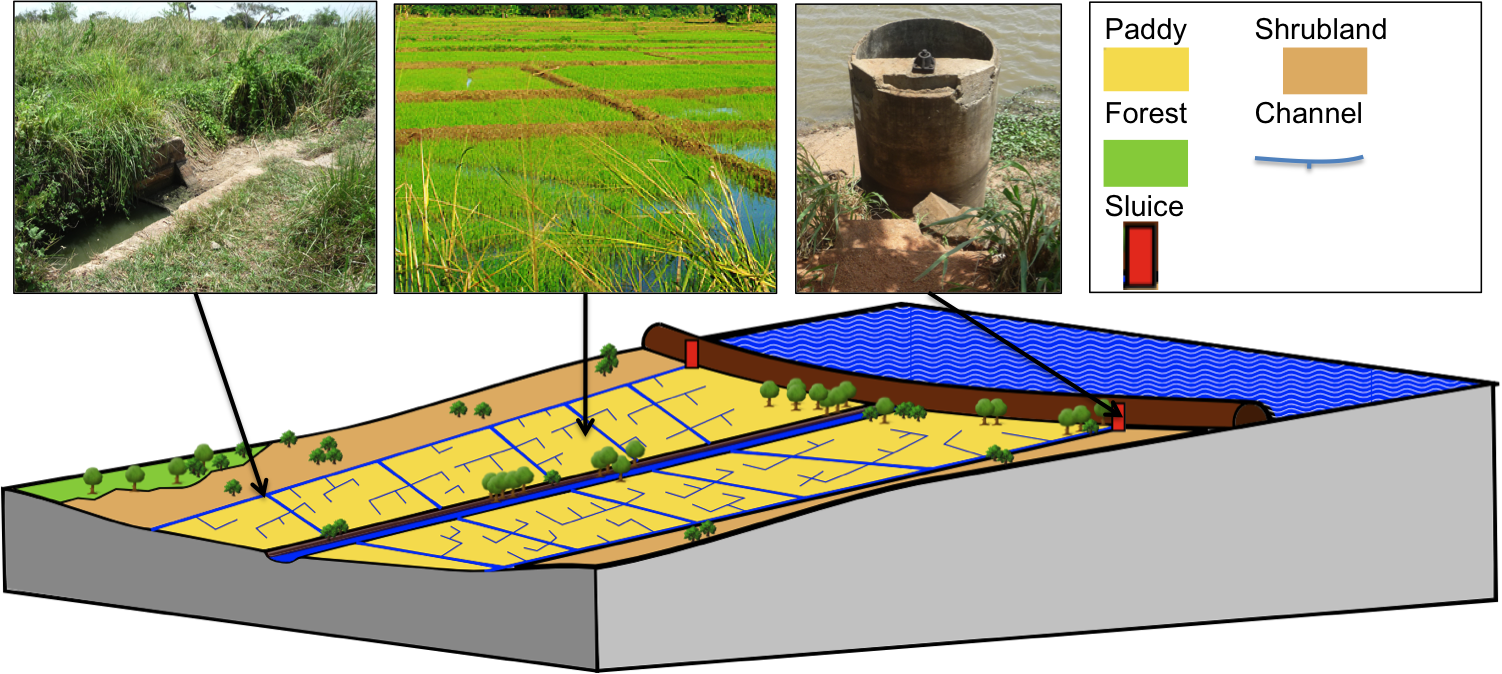
\includegraphics[width=0.8\textwidth]{images/Beispiel.png} % 0.8/textwidth setzt das Bild in 0,8-facher Textbreite. Der Faktor kann variiert oder weggelassen werden. Es gibt auch \textheight! Beachte bei Karten mit Maßstab, dass dieser beim Skalieren verändert wird!
\caption[Bildunterschrift für das Abb.Verz.]{Bildunterschrift \citep[aus:][]{nachname_2005}}
\label{fig:Beispiel.png} % Gibt man im Text \ref{fig:Beispiel.png} an, wir dort automatisch die Nummer des Bildes gesetzt.
\end{figure}



\subsection{Unterkapitel 2}

Lorem ipsum dolor sit amet, consetetur sadipscing elitr, sed diam nonumy eirmod tempor invidunt ut labore et dolore magna aliquyam erat, sed diam voluptua. At vero eos et accusam et justo duo dolores et ea rebum. Stet clita kasd gubergren, no sea takimata sanctus est Lorem ipsum dolor sit amet. Lorem ipsum dolor sit amet, consetetur sadipscing elitr, sed diam nonumy eirmod tempor invidunt ut labore et dolore magna aliquyam erat, sed diam voluptua. At vero eos et accusam et justo duo dolores et ea rebum. Stet clita kasd gubergren, no sea takimata sanctus est Lorem ipsum dolor sit amet. Lorem ipsum dolor sit amet, consetetur sadipscing elitr, sed diam nonumy eirmod tempor invidunt ut labore et dolore magna aliquyam erat, sed diam voluptua. At vero eos et accusam et justo duo dolores et ea rebum. Stet clita kasd gubergren, no sea takimata sanctus est Lorem ipsum dolor sit amet.   

\subsubsection{Unterunterkapitel}
